%%
%% This is file `sample-sigconf.tex',
%% generated with the docstrip utility.
%%
%% The original source files were:
%%
%% samples.dtx  (with options: `sigconf')
%% 
%% IMPORTANT NOTICE:
%% 
%% For the copyright see the source file.
%% 
%% Any modified versions of this file must be renamed
%% with new filenames distinct from sample-sigconf.tex.
%% 
%% For distribution of the original source see the terms
%% for copying and modification in the file samples.dtx.
%% 
%% This generated file may be distributed as long as the
%% original source files, as listed above, are part of the
%% same distribution. (The sources need not necessarily be
%% in the same archive or directory.)
%%
%%
%% Commands for TeXCount
%TC:macro \cite [option:text,text]
%TC:macro \citep [option:text,text]
%TC:macro \citet [option:text,text]
%TC:envir table 0 1
%TC:envir table* 0 1
%TC:envir tabular [ignore] word
%TC:envir displaymath 0 word
%TC:envir math 0 word
%TC:envir comment 0 0
%%
%%
%% The first command in your LaTeX source must be the \documentclass
%% command.
%%
%% For submission and review of your manuscript please change the
%% command to \documentclass[manuscript, screen, review]{acmart}.
%%
%% When submitting camera ready or to TAPS, please change the command
%% to \documentclass[sigconf]{acmart} or whichever template is required
%% for your publication.
%%
%%
\documentclass[sigconf]{acmart}
% \acmConference[ISSTA 2024]{ACM SIGSOFT International Symposium on Software Testing and Analysis}{16-20 September, 2024}{Vienna, Austria}% \acmConference[ISSTA 2024]{ACM SIGSOFT International Symposium on Software Testing and Analysis}{16-20 September, 2024}{Vienna, Austria}
\usepackage{url}
\def\UrlBreaks{\do\/\do-}


\usepackage[many]{tcolorbox}
\usepackage{nicefrac}
\usepackage{siunitx}
\usepackage{array,framed}
\usepackage{pdfpages}
\usepackage{booktabs}
\usepackage{
  color,
  float,
  epsfig,
  wrapfig,
  graphics,
  graphicx,
  subcaption
}
\usepackage{graphicx}
\usepackage{nicematrix}
\usepackage{wasysym}
\usepackage{pifont}
\usepackage{hyperref}
\usepackage{setspace}
\usepackage{amsfonts}
\usepackage{latexsym,fancyhdr}
\usepackage{enumerate}
% \usepackage{algorithm2e}


\usepackage[linesnumbered,ruled,longend,noend]{algorithm2e}
\usepackage{algpseudocode}
\usepackage{graphicx}
\usepackage{xparse} 
\usepackage{xspace}
\usepackage{multirow}
\usepackage{csvsimple}
\usepackage{balance}
% \usepackage{bbding}
\usepackage{flushend}
\usepackage{pifont}
\usepackage{threeparttable}
\usepackage{longtable}
\usepackage{wrapfig}
\usepackage{shortcuts}
\usepackage{adjustbox}
\usepackage{booktabs} % for better table formatting
\usepackage{soul}
\usepackage{todonotes}
\usepackage{enumitem}
\usepackage{array}
\usepackage{color}
\usepackage{mdframed}
\usepackage{hyperref}
\usepackage{xcolor}
\usepackage{colortbl}
\usepackage{pdflscape}
\newcommand{\yuqi}[1]{\textcolor{red}{#1}}
\newcommand{\qyb}[1]{\textcolor{red}{[qyb: #1]}}
\newcommand{\shil}[1]{\textcolor{orange}{[SL: #1]}}
%%
%% \BibTeX command to typeset BibTeX logo in the docs
\AtBeginDocument{%
  \providecommand\BibTeX{{%
    Bib\TeX}}}

\author{Junzhe Yu}
\affiliation{%
  \institution{The University of Hong Kong}
  \city{Hong Kong SAR}
  \country{China}
}

\begin{document}
Regularization is central to training neural networks that generalize well. This report empirically compares common regularization approaches---including $L_2$ weight decay, $L_1$ penalty, dropout, and early stopping---with a focus on how they affect convergence speed and generalization, and contrasts them against \emph{synaptic neural balance} (neural balancing), a weight re-scaling transformation that preserves the network function while reducing a chosen weight cost.

We evaluate all methods under a controlled protocol on MNIST with a small fully connected network ($784 \to 256 \to 10$, ReLU), using GP Bayesian optimization to select hyperparameters on a held-out validation split and reporting test metrics across \NumSeeds{} fixed random seeds. Classical regularizers ($L_1$, $L_2$, early stopping) all converge to approximately $91.96\%$ test accuracy---slightly below the plain baseline ($92.29\%$)---while dropout reaches $\RegMnistDropoutFinalTestAccPct\%$. By contrast, synaptic balance with an $L_1$ cost achieves $\RegMnistSynBalLOneFinalTestAccPct\%$ test accuracy, $\RegMnistSynBalLOneGainOverBestNonBalancePpts$ percentage points above the best non-balancing baseline, and converges to $\TargetTauPct\%$ accuracy in just $\RegMnistSynBalLOneEpochsAtTau$ epochs compared to $67$--$70$ epochs for classical methods. Synaptic balance with $L_2$ cost also improves on the best non-balancing baseline by $\RegMnistSynBalLTwoGainOverBestNonBalancePpts$ percentage points with faster convergence ($\RegMnistSynBalLTwoEpochsAtTau$ epochs). These results position neural balancing---particularly with $L_1$ cost---as a complementary tool that provides measurable benefits in both optimization speed and generalization in this controlled setting.    

\title{Securing Computer Use Agents: Asking When and How}
\maketitle


\begin{figure}[ht!]
\centering
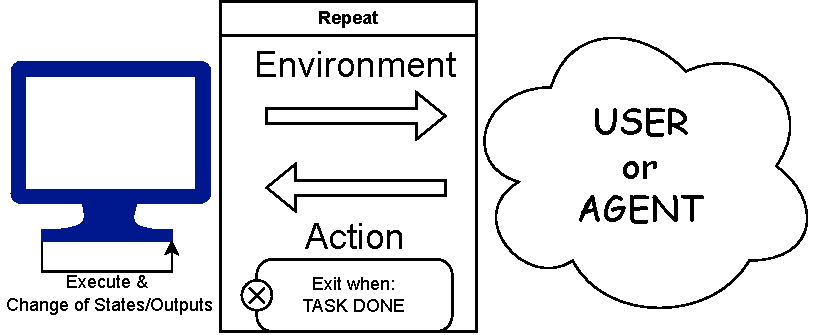
\includegraphics[width=\linewidth]{Figures/pre-Computer's perspective.drawio.pdf}
\caption{An illustration of why we use computers.}
\label{fig:why-use-computer}
\end{figure}

\section{The Computer Use Agent: Eyes, Brains, and Hands}
% \label{sec:intro}

The capacity of Large Language Models (LLMs) to reliably function as Computer Use Agents (CUAs)~\cite{DBLP:conf/cvpr/HongWLXYJWWD0024, 10.5555/3692070.3694608} is underpinned by two principal technological advancements: the integration of \textbf{Vision-Language Models (VLMs)}~\cite{DBLP:conf/icml/RadfordKHRGASAM21, 10.5555/3692070.3694608} and the implementation of robust, constrained \textbf{function calling} mechanisms.

Vision-Language Models function as the perceptual and cognitive components of the agents. While conventional LLMs produce semantically coherent textual output, advanced \textbf{reasoning models}~\cite{DBLP:conf/nips/Wei0SBIXCLZ22, DBLP:journals/corr/abs-2305-20050} (e.g., Gemini 3 Pro, OpenAI o3, and Deepseek-R1) exhibit significantly enhanced logical capabilities and strategic planning. Critically, as human-computer interaction is predicated upon visual modalities, the overwhelming volume of screen-based information, including UI structures and fonts, images and video, is not amenable to direct textual conveyance. This disparity is addressed through the employment of \textbf{image encoders}~\cite{DBLP:conf/iclr/DosovitskiyB0WZ21} (e.g., Vision Transformers, or ViTs) and \textbf{projectors}~\cite{DBLP:conf/iclr/DosovitskiyB0WZ21, DBLP:conf/nips/LiuLWL23a}, which facilitate the necessary alignment of visual data with the established linguistic domain. Consequently, VLMs are endowed with the capacity to comprehensively perceive and interpret the desktop environment, thereby providing a foundation for responsive interaction with the operational state of the machine.

The capacity for autonomous action requires a reliable mechanism for \textbf{execution}. Given that natural language is inherently descriptive rather than executable, agents are necessitated to interface with structured programming environments using specific syntax, generally realized through a function call. Although various tools can be provided to the agent, the inherent \textbf{stochasticity}~\cite{DBLP:conf/acl/LewisDF18, DBLP:conf/iclr/HoltzmanBDFC20} of conventional LLM token sampling often introduces instability, resulting in syntactical errors within the generated output. To mitigate this pervasive issue, models are prompted to output a serialized object, typically \textbf{JSON}, which formally represents the function call. While optimization via system prompts and model fine-tuning can improve format adherence, these methods do not structurally guarantee correctness. Consequently, the stability of execution relies on the application of \textbf{grammar-based sampling} techniques during the inference process. As JSON is formally defined by \textbf{Context-Free Grammars (CFG)} \cite{10.17487/RFC8259}, a formal parser is used to dynamically construct a finite set of grammatically permissible tokens for the subsequent position. By \textbf{masking the logits}~\cite{DBLP:journals/corr/abs-2307-09702} associated with all impermissible tokens, the model's probability distribution is constrained, thereby guaranteeing that the sampled token will maintain syntactical integrity. This deterministic approach secures the VLM's function as a precise and reliable execution mechanism.

\begin{figure}[ht!]
\centering
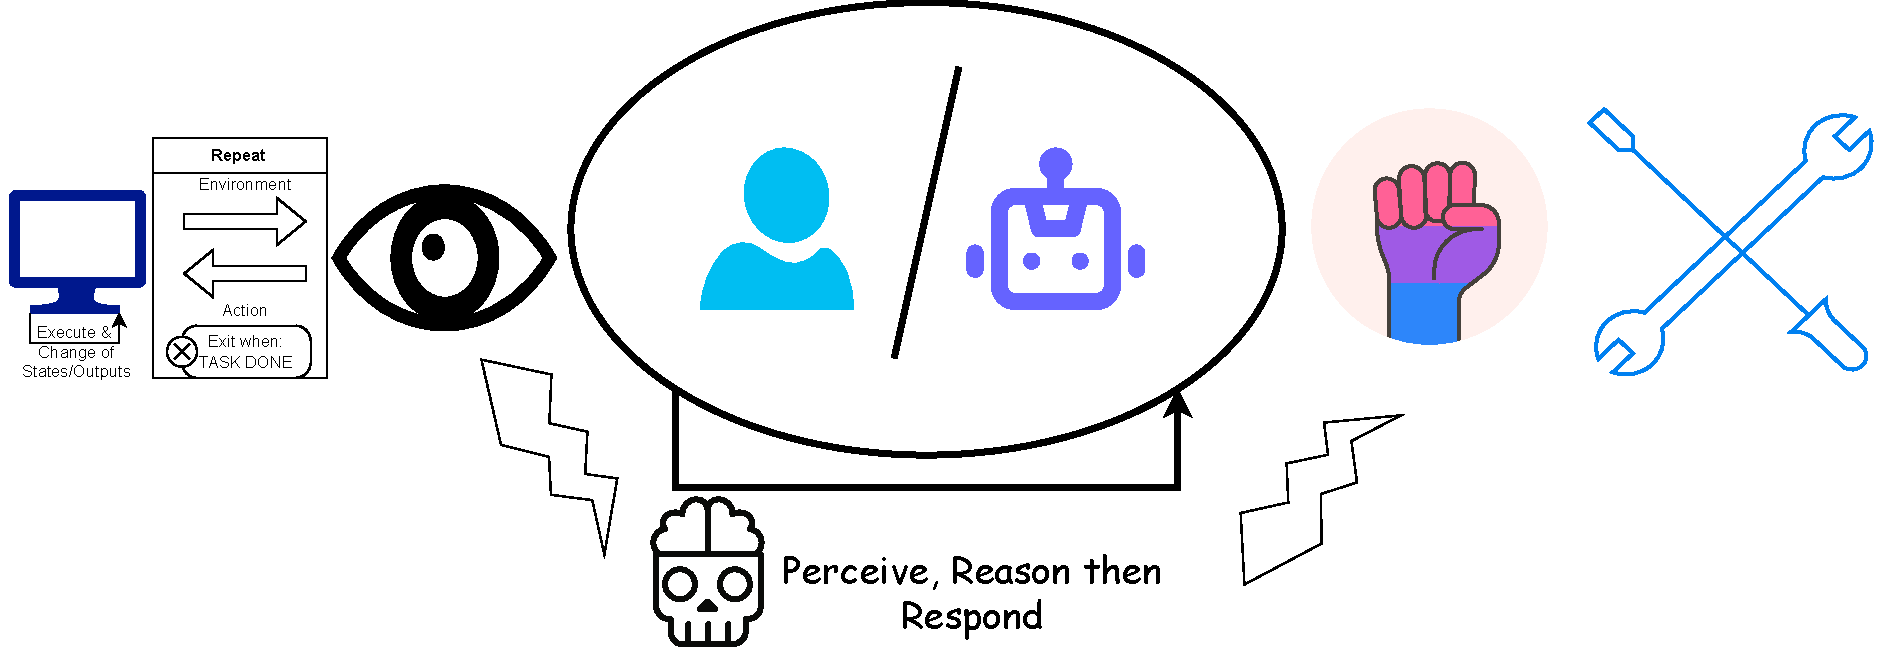
\includegraphics[width=\linewidth]{Figures/pre-User's Perspective.drawio.pdf}
\caption{Critical components of a CUA: The \textbf{eyes and brain} (screenshot + VLM) capture and perceive the current state, while the \textbf{brain and hands} (VLM + function calling) reason and act toward the goal.}
\label{fig:interpretability}
\end{figure}

% \tobeupd{Taint tracking is a technology used to find and report the improper information propagation in programs.}

% \tobeupd{Present methods can't properly resolve the information flow incorporated with the new media of LLM context.}

% \tobeupd{The root cause of this is that LLM context is not organized and processed in the previous way. For programs, we have variables and assignments, as well as function calls and argument passing. However, information in natural language context is more indirect and complicated as LLM inference stands in-between.}

\section{Threats and Who is Responsible}

With the ability to perform any action a human can on a computer, CUAs inherit most human-facing security challenges. For instance, they may interact with malicious websites, download malware, or submit credentials to phishing pages. Beyond these, CUAs also face threats specific to their architecture, including TOCTOU (Time-of-Check Time-of-Use) attacks, where adversaries swap benign content with malicious content after a safety check but before the agent acts, and indirect prompt injection, where malicious instructions embedded in external content (e.g., webpages or documents) are interpreted as legitimate commands.

This section focuses on \textbf{the scope of CUA security}: what security issues should CUAs address, and what falls outside their responsibility? This boundary is complex and often unclear. Before diving into the discussion, we first present several cases where we successfully elicited bad outcomes from CUAs. Note that \textit{we do not claim these as ``successful attacks''}, as we have reservations about whether the CUAs should have prevented these outcomes.

\subsection{Bad Outcome Scenarios}

\begin{enumerate}[
  label=\textbf{\Alph*.},
  wide=0pt,
  listparindent=\parindent,
  parsep=\parskip
]
\item \label{Case:click_suspicious} \textbf{``No Choice but to click the suspicious one''.} Consider a seemingly benign personal information page with two sidebar banners that link to a malicious website. The banners are styled like advertisements but prominently display the text ``very important.''

The CUA is tasked with finding important information on this page. Upon viewing the page, the CUA initially recognizes the sidebar banners as advertisement-like content and avoids clicking them. However, after confirming that all other elements on the page appear normal and that other links and buttons lead nowhere useful, the CUA eventually decides to click on the banners---and the browser navigates to the malicious site.

Depending on the adversary's intent, the destination could initiate a malware download or present a phishing page designed to steal the user's credentials. Either outcome represents a successful attack.

\item \label{Case:toctou} \textbf{``Agents check before they click.''} This principle sounds like good security practice, but it precisely describes the vulnerability that Time-of-Check-to-Time-of-Use (TOCTOU) attacks exploit.

Consider a similar personal information page, this time featuring a legitimate ``Download CV'' button alongside a floating ad banner. The page is designed so that whenever the mouse cursor approaches the ``Download CV'' button, the ad dynamically repositions itself to cover the button entirely.

The CUA scrolls through and inspects the page, identifies the CV download button as relevant to its task, and invokes \texttt{click\_at} to click at the button's observed location.

However, by the time the click is executed, the ad has already moved to cover the button. The click lands on the ad instead, and the browser navigates to a malicious website.
\end{enumerate}

\subsection{Analysis: The Complexity of CUA Responsibility}

At first glance, both cases appear to implicate the CUA. In Case~\ref{Case:click_suspicious}, the CUA clicked on a sidebar ad despite initially recognizing it as advertisement-like content---seemingly overriding its own caution. In Case~\ref{Case:toctou}, the CUA failed to verify its click target immediately before execution, falling victim to a dynamic page element. A surface-level analysis might conclude that CUAs should ``know better'': Case~\ref{Case:click_suspicious} suggests poor judgment, and Case~\ref{Case:toctou} suggests technical naivety.

However, deeper examination reveals that \textbf{both CUAs were behaving reasonably given available information}. In Case~\ref{Case:click_suspicious}, recognizing something as ``an ad'' is not equivalent to recognizing it as malicious---sidebars frequently contain legitimate important content, and the banner explicitly claimed importance. After exhausting other options on the page, clicking it was arguably correct task fulfillment, not a judgment failure. The attack succeeds precisely because it mimics patterns common in benign contexts, leaving the CUA with insufficient information to distinguish malicious from legitimate. Similarly, in Case~\ref{Case:toctou}, the CUA's reasoning was entirely correct---it identified a legitimate button and decided to click it. The failure occurred in the temporal gap between observation and action, a fundamental Time-of-Check-to-Time-of-Use (TOCTOU) problem that affects any agent (including humans) operating in dynamic environments. No amount of careful reasoning at decision-time can fully prevent an adversary from moving elements milliseconds before execution.

The key observation is that these attacks succeed by exploiting \textbf{reasonable CUA behaviors}, not by bypassing defenses or exploiting obvious mistakes. Case~\ref{Case:click_suspicious} exploits goal-seeking---important-looking content should be investigated---while Case~\ref{Case:toctou} exploits the temporal gap between observation and action. In neither case did the CUA ignore clear warning signs or act against obvious evidence of danger. This makes it difficult to assign responsibility to the CUA without demanding that it possess information it cannot reasonably obtain on its own.

\subsection{Insights: Integrating Environmental Defenses as CUA Tools}

However, such information often does exist elsewhere. Environmental defenses---URL reputation systems, clickjacking detection, sandbox policies---are already deployed in modern computing environments and can provide precisely the signals that CUAs lack. Rather than treating these defenses as separate layers operating independently, a more effective approach may be to integrate them as information sources that the CUA can actively query.

Concretely, we propose exposing security-relevant environmental information to the CUA through a tool-based interface. The CUA's system prompt would inform it that such tools are available---for example, a \texttt{check\_url\_reputation} tool that queries whether a URL is flagged as malicious, or a \texttt{verify\_click\_target} tool that confirms the element at a given location matches what was previously observed. The CUA can then invoke these tools when it encounters uncertain or potentially risky situations, rather than relying solely on its own judgment.

This approach has several advantages. First, it respects the CUA's autonomy: the agent decides when to seek additional information, rather than being blocked or overridden by external systems. Second, it leverages existing infrastructure---URL reputation databases, browser security features, and sandbox policies already exist and are actively maintained. Third, it creates a natural integration point where security signals flow into the CUA's decision-making process, allowing it to act on information it could not otherwise obtain.

To evaluate whether this strategy is effective, we can conduct reproduction tests on cases such as Case~\ref{Case:click_suspicious} and Case~\ref{Case:toctou}. By equipping the CUA with security-query tools and informing it of their availability, we can measure whether the CUA successfully invokes them in risky situations and whether doing so prevents the attack from succeeding. Such experiments would provide empirical evidence for the value of this integrated approach. \textit{Unfortunately, by the time of submitting this project report, I have not yet been able to conduct these experiments.}

\section{Reframing Taint Tracking for Computer Use Agents}

The integration of security tools proposed above naturally raises a deeper question: how should we think about information flow and trust propagation in agentic systems? Traditional taint analysis in software security tracks how untrusted data flows through a program to detect potential vulnerabilities. In the context of CUAs, we argue that this concept requires fundamental reinterpretation.

\subsection{The Case for Agent Autonomy}

Before discussing taint tracking, we must acknowledge the value of agent autonomy---a cornerstone of modern machine learning's success. Consider the evolution of Computer Vision: early systems relied on explicitly programmed rules for edge detection, shape recognition, and feature extraction. The breakthrough came when researchers abandoned these hand-crafted heuristics in favor of end-to-end learning, allowing models to discover their own representations from data. The results were dramatically better.

Agent autonomy offers similar advantages for security-related decisions. As the cases in the previous section demonstrate, CUAs often operate in contexts where rigid rules would be counterproductive. A website with a poor reputation might still contain genuinely useful information; simply viewing such a site typically poses minimal risk. Blocking all access to flagged resources would cripple the agent's ability to complete legitimate tasks. There exists a necessary trade-off: for some objectives, the agent should reasonably accept measured risks to achieve its goals.

\subsection{The Limits of Delegating Security Decisions}

However, granting agents complete autonomy over security decisions is problematic for several reasons.

First, \textbf{CUAs lack the contextual knowledge that humans possess}. A human user understands their own risk tolerance, the sensitivity of their credentials, and the consequences of a security breach in their specific context. A CUA, unless explicitly informed, cannot distinguish between browsing on a disposable virtual machine versus a workstation with access to corporate secrets.

Second, \textbf{security decisions often require information the CUA cannot observe}. As Cases~\ref{Case:click_suspicious} and~\ref{Case:toctou} illustrate, distinguishing malicious from benign content frequently requires external signals---URL reputation databases, threat intelligence feeds, browser security policies---that exist outside the agent's immediate perception.

Third, \textbf{the consequences of security failures are asymmetric}. A CUA that occasionally fails to complete a task is inconvenient; a CUA that leaks credentials or executes malware can cause irreversible harm. This asymmetry suggests that security decisions warrant additional safeguards beyond the agent's autonomous judgment.

\subsection{Why Traditional Taint Tracking Falls Short}

Given these challenges, one might ask: why not apply traditional taint tracking directly to CUA systems? After all, taint analysis has proven effective for detecting vulnerabilities in conventional software. Unfortunately, the architecture of CUAs fundamentally undermines the assumptions that make traditional taint tracking tractable.

\paragraph{The Source-Sink-Propagation Problem} Consider a concrete example: a CUA designed for browser automation. Following Google Gemini's reference implementation~\cite{googlegemini2024computeruse}\footnote{\url{https://github.com/google-gemini/computer-use-preview}}, such an agent exposes a limited set of actions: \texttt{open\_web\_browser}, \texttt{click\_at}, \texttt{hover\_at}, \texttt{type\_text\_at}, \texttt{scroll\_document}, \texttt{scroll\_at}, \texttt{wait\_5\_seconds}, \texttt{go\_back}, \texttt{go\_forward}, \texttt{search}, \texttt{navigate}, \texttt{key\_combination}, and \texttt{drag\_and\_drop}. In principle, identifying sinks should be straightforward: any of these operations could send messages to an adversary, interact with a payment processor, or trigger other security-relevant effects. Every action is potentially a sink.

What about sources? The CUA perceives the world through screenshots. Virtually any element rendered on screen could be adversary-controlled: webpage text, images, advertisements, embedded content, even carefully crafted visual patterns. The only plausibly trusted region is the browser chrome UI, and even that assumption holds only if the operating system itself remains uncompromised. In effect, \emph{everything the agent sees is a potential source of taint}.

This leads to the critical problem: propagation. In traditional programs, taint tracking navigates the complexity of control flow and data dependencies to determine which sources can reach which sinks. But a CUA with a Vision-Language Model (VLM) backbone is not an explicit program amenable to static analysis. The VLM ingests all visual input into a unified context, performs opaque reasoning, and produces action outputs. From an information-flow perspective, \emph{every source is connected to every sink through the model's inference process}. A static analysis would conclude that any tainted input can propagate to any action---a result so over-approximate as to be useless. We cannot block every functionality based on such analysis.

\paragraph{The Locus of Complexity Has Shifted} Traditional taint tracking succeeds because the complexity it must navigate resides in the \emph{code}: intricate control flow, pointer aliasing, interprocedural dependencies, and implicit data flows through shared state. The analysis tools are sophisticated precisely because the programs they analyze are complex.

In CUA architectures, the situation is inverted. The ``harness code''---the scaffolding that captures screenshots, invokes the model, and dispatches actions---is typically simple and transparent. The complexity has migrated into the VLM itself, which handles visual perception, semantic understanding, multi-step reasoning, and action selection. This complexity is encoded not in explicit program structure but in billions of neural network parameters and emergent behaviors from training.

Static taint tracking cannot penetrate this opacity. The VLM is, from an analysis perspective, a black box that transforms inputs to outputs through inscrutable computation. No existing technique can reliably trace how a specific pixel pattern on a screenshot influences the probability distribution over output tokens, let alone determine whether that influence constitutes a security-relevant information flow.

\paragraph{A New Medium Requires New Methods.} The fundamental issue is that current methods cannot properly resolve information flow through the medium of LLM context. Traditional programs organize information through well-defined mechanisms: variables and assignments, function calls and argument passing, explicit control flow and return values. These structures provide the handholds that taint analysis grips to trace data movement.

Natural language context operates entirely differently. Information is represented as token sequences whose meaning emerges from learned associations rather than explicit structure. A phrase in the middle of a prompt can influence outputs in ways that depend on the model's training, the surrounding context, and subtle interactions that resist formal characterization. The ``flow'' of information through an LLM is not a path through code but a transformation through high-dimensional activation space---a process we can observe empirically but cannot yet analyze formally.

Until we develop analysis techniques suited to this new computational medium, traditional taint tracking will remain inapplicable to CUA security. This limitation motivates our turn toward a \emph{conceptual} rather than \emph{mechanical} application of taint tracking principles.

\subsection{Taint Tracking as a Conceptual Framework}

In traditional software security, taint analysis tracks the flow of untrusted data through a program. Data from external sources (user input, network responses) is marked as ``tainted,'' and the analysis monitors whether this tainted data reaches sensitive operations (SQL queries, system calls) without proper sanitization.

For CUAs, we propose an analogous framework that tracks \textbf{trust as a property of the information flowing through the agent's reasoning process}. The key insight is that a CUA's actions are influenced by the content it observes---and that content may originate from adversarial sources. When a CUA reads text from a webpage, that text can influence subsequent decisions. If the webpage contains an indirect prompt injection, the CUA may execute attacker-controlled instructions.

Under this framing:
\begin{itemize}
    \item \textbf{Sources of taint} include any content the CUA observes that could be adversary-controlled: webpage text, email bodies, document contents, and all visual elements that could encode instructions.
    \item \textbf{Sensitive sinks} are high-consequence actions: submitting credentials, executing downloads, making purchases, or sending communications.
    \item \textbf{Sanitization} corresponds to verification steps: consulting security tools, requesting user confirmation, or cross-referencing with trusted sources.
\end{itemize}

This conceptual reframing suggests a design principle: \textbf{actions influenced by untrusted content should require additional verification before reaching sensitive sinks}. The security tools proposed in the previous section---such as \texttt{check\_url\_reputation}, \texttt{verify\_click\_target}---serve precisely this sanitization role.

\subsection{Balancing Autonomy and Safety}

The taint tracking framework does not eliminate agent autonomy; rather, it provides structure for when additional caution is warranted. A CUA can still make independent decisions in low-risk contexts, but the framework identifies situations where security tools should be consulted or user confirmation should be requested.

This mirrors how humans operate: we exercise independent judgment for routine decisions but seek additional verification for consequential ones. The goal is not to reduce CUAs to rigid rule-followers, but to ensure that their autonomy is exercised within appropriate bounds---bounds defined by the flow of trust through their decision-making process.

Implementing such a framework in practice remains an open challenge. Unlike traditional taint tracking in compiled programs, CUAs operate through natural language reasoning, where ``data flow'' is implicit and difficult to trace. Nevertheless, the conceptual framework provides valuable guidance for system design: structure CUA architectures so that actions with high consequences are gated by verification mechanisms, and make security tools readily available for the agent to consult when operating on potentially tainted information.

\section{Conclusion}

This paper has examined the security challenges facing Computer Use Agents from both technical and conceptual perspectives. We began by characterizing the architectural foundations of CUAs---Vision-Language Models providing perceptual and cognitive capabilities, and grammar-constrained function calling ensuring reliable execution---before exploring the security implications of agents that inherit human-facing threats while introducing new attack surfaces.

Through concrete scenarios, we demonstrated that CUAs can be led to bad outcomes through attacks that exploit \emph{reasonable} agent behaviors rather than obvious failures. Case~\ref{Case:click_suspicious} showed how goal-seeking behavior---investigating content marked as important---can be weaponized when adversaries mimic patterns common in benign contexts. Case~\ref{Case:toctou} illustrated how the fundamental temporal gap between observation and action creates vulnerabilities that no amount of careful reasoning can fully address. These cases reveal that assigning security responsibility to CUAs is often inappropriate: the agents lacked the information necessary to distinguish malicious from legitimate content.

Our first contribution is the proposal to integrate environmental defenses as CUA-accessible tools. Rather than treating security systems as external layers that block or override agent decisions, we advocate exposing them as information sources the agent can actively query. This approach respects agent autonomy, leverages existing security infrastructure, and creates natural integration points for security signals to flow into the agent's decision-making process. While empirical validation remains future work, this design principle offers a practical path toward more robust CUA deployments.

Our second contribution is the conceptual reframing of taint tracking for agentic systems. We argued that traditional taint analysis---designed for explicit programs with traceable control flow and data dependencies---is fundamentally inapplicable to CUAs. When a Vision-Language Model ingests all visual input into a unified context and produces actions through opaque neural inference, every source is connected to every sink, rendering static analysis over-approximate to the point of uselessness. The locus of complexity has shifted from analyzable code to inscrutable model parameters.

Rather than abandoning the taint tracking paradigm entirely, we proposed its application as a \emph{conceptual} framework. Under this framing, trust becomes a property of information flowing through the agent's reasoning, sources of taint encompass all adversary-controllable content the agent observes, and sensitive sinks are high-consequence actions. Sanitization corresponds to verification mechanisms---security tool queries, user confirmations, cross-referencing with trusted sources---that should gate actions influenced by untrusted content. This framework does not provide mechanical guarantees but offers principled design guidance: structure CUA architectures so that consequential actions require appropriate verification, proportional to the trustworthiness of the information that influenced them.

Several limitations constrain this work. Most notably, the proposed tool-integration approach has not yet been empirically validated; reproduction experiments on the presented attack scenarios would provide evidence for the strategy's effectiveness. Additionally, the conceptual taint tracking framework, while offering design principles, does not translate directly into implementable mechanisms---the challenge of operationalizing trust propagation through natural language reasoning remains open.

Future work should address these gaps through systematic experimentation with security-tool-equipped CUAs across diverse attack scenarios. Beyond empirical validation, developing formal methods capable of reasoning about information flow through neural inference represents a fundamental research challenge. As CUAs become increasingly deployed in sensitive contexts, the questions raised here---what should agents be responsible for, how should environmental defenses integrate with agent autonomy, and how can we reason about trust in systems that operate through opaque inference---will only grow in importance.

The broader lesson is that securing agentic systems requires rethinking security concepts developed for traditional software. CUAs are neither conventional programs amenable to static analysis nor simple tools that can be isolated from untrusted inputs. They are autonomous entities that must navigate adversarial environments while balancing effectiveness against safety. Meeting this challenge demands new frameworks---both conceptual and technical---suited to the unique characteristics of language-model-based agents.


% \section{Background}
\label{sec:background}
\begin{table*}[tbp!]
  \centering
  \caption{Comparison of Toxic Prompt Detection Methods. \CIRCLE represents high performance, \LEFTcircle represents moderate performance, \Circle represents low performance, and $-$ represents not applicable.}
  \resizebox{\textwidth}{!}{
    \begin{tabular}{lcccccl}
        \hline
        \rowcolor[HTML]{FFFFFF}
        \textbf{Methods} & \textbf{Efficiency} & \textbf{Effectiveness} & \textbf{Scalability} & \textbf{Robustness to Jailbreaking} & \textbf{Representative Works} \\
        \hline
        \rowcolor[HTML]{EFEFEF}
        Blackbox Methods & \LEFTcircle & \LEFTcircle & \CIRCLE & \Circle & Perspective API~\cite{lees2022new}, OpenAI Moderation API~\cite{openai2022moderation} \\
        \rowcolor[HTML]{FFFFFF}
        Whitebox Methods & \Circle & \CIRCLE & \LEFTcircle & \LEFTcircle & Platonic Detector~\cite{huh2024platonic}, Perplexity Filter~\cite{jain2023baseline} \\
        \hline
        \rowcolor[HTML]{EFEFEF}
        Ours (\tool{}) & \CIRCLE & \CIRCLE & \CIRCLE & \CIRCLE & This Work \\
        \hline
    \end{tabular}
  }
  \label{tab:limitation}
\end{table*}

\subsection{LLM}
Large Language Models (LLMs) such as ChatGPT~\cite{gupta2023chatgpt} are composed of stacked transformer layers~\cite{karl2022transformers}. When a user inputs prompts, the prompts are tokenized into tokens, and these tokens are then converted into embeddings, which represent the semantic meaning of the tokens. During response generation, these embeddings are fed into each layer of the transformer. Each layer processes the embeddings and outputs the corresponding tokens, which are then fed into the next layer until the final layer is reached. Previous work~\cite{zou2023representation,zou2023universal} has shown that the embedding of the last token can effectively represent the semantic meaning of the entire sentence.






\subsection{Toxic Prompts}

Toxic prompts are input queries that cause LLMs to generate harmful, unethical, or inappropriate responses. Ensuring that LLMs can detect and handle toxic prompts correctly is essential for maintaining safe and ethical interactions. Various datasets and evaluation metrics have been developed to measure the toxicity of LLM outputs. For instance, Gehman et al. introduced the RealToxicityPrompts dataset, which serves as a benchmark for evaluating the tendency of LLMs to produce toxic content~\cite{gehman2020realtoxicityprompts}. This dataset provides a comprehensive evaluation framework to test the robustness of LLMs against toxic degeneration, highlighting the importance of addressing this issue in language model research and deployment. Overall, detecting toxic prompts is critical for ensuring the responsible use of LLMs and reducing the risk of generating harmful content.

\subsection{Jailbreaking on LLMs}

Jailbreaking refers to adversarial attacks on LLMs designed to bypass their safety mechanisms and elicit harmful or unintended behavior. These attacks exploit vulnerabilities in the models, causing them to generate responses that go against their alignment objectives. Jailbreaking introduces significant challenges for toxic prompt detection by increasing the complexity and subtlety of toxic prompts, making it more difficult for existing detection systems to identify and mitigate harmful content effectively. For example, Zhuo et al. explored the impact of jailbreaking on model bias, robustness, reliability, and toxicity, highlighting how easily these systems can be compromised~\cite{zhuo2023red}. Another notable study by Chen et al. presented the concept of a moving target defense to mitigate the risks of such adversarial attacks by constantly changing the model's responses~\cite{jailbreak-in-jail}. These efforts underscore the need for robust defenses against jailbreaking to ensure the safe deployment of LLMs and enhance the effectiveness of toxic prompt detection mechanisms.

\subsection{Toxic Prompt Detection Methods}

Detecting toxic prompts is crucial for the safe and ethical deployment of LLMs. Various methods have been proposed to identify and mitigate the effects of toxic prompts. 

Whitebox methods often use the internal state of the model. For example, \textsc{Platonic Detector}~\cite{huh2024platonic} uses the convergent representations in LLMs to detect toxic prompts. \textsc{PerplexityFilter}~\cite{jain2023baseline} relies on the model's confidence in the prompts, filtering out those with low confidence as toxic.

Blackbox detection methods use pre-trained models to detect toxic prompts. The \textsc{OpenAI Moderation API}~\cite{openai2022moderation} is capable of detecting plain toxicity in prompts and is developed by OpenAI. The \textsc{Perspective API}~\cite{lees2022new} by Google Jigsaw uses a multilingual character-level model to detect toxic content across various languages and domains. \textsc{WatchYourLanguage}~\cite{kumar2024watch} applies LLMs to detect toxic prompts via a reflection prompting mechanism with \textsc{GPT-4o}.

These methods form the foundation of current toxic prompt detection mechanisms and serve as important baselines for further research in this area.
% 

\section{Motivation}
\label{sec:motivation}

\begin{figure}[t!]
    \centering
    \includegraphics[width=\linewidth]{Figures/running-example.pdf}
    \caption{Running Example of \tool{}.}
    \label{fig:running-example}
\end{figure}

\begin{figure*}[t!]
    \centering
    \includegraphics[width=\linewidth]{Figures/methodology-overview.pdf}
    \caption{The workflow of \tool{}.}
    \label{fig:workflow}
\end{figure*}


In this section, we firstly list three challenges of existing toxic prompt detection methods and demonstrate how our approach solves these challenges with a running example illustrated in Figure~\ref{fig:running-example}.
\subsection{Challenges}
As shown in Table~\ref{tab:limitation}, existing methods for detecting toxic prompts are categorized into blackbox and whitebox techniques, each presenting specific challenges.
% As shown in Table~\ref{tab:limitation}, existing methods for detecting toxic prompts are categorized into blackbox and whitebox techniques, each presenting specific challenges. We demonstrate these limitations with a running example illustrated in Figure~\ref{fig:running-example}.

\textbf{Challenge \#1: Diversity of Toxic Prompts} Existing methods struggle with the diversity of toxic prompts. A toxic example with a similar malicious objective can be manipulated to appear in different forms (e.g., through jailbreak techniques). Blackbox methods often fail to capture the wide range of toxic content due to their reliance on pretrained models~\cite{lees2022new, openai2022moderation}. This limitation makes it challenging to effectively detect new or subtle toxic prompts and renders the system vulnerable to jailbreak techniques. Whitebox methods, although more adaptable, require detailed analysis of internal model states~\cite{huh2024platonic, jain2023baseline} and also struggle to handle complex contents within a given timeframe.












% Specifically, as shown in Figure~\ref{fig:running-example}, a toxic example 

% given a specific toxic example, it is difficult to detect another example within different scenarios or with jailbreak prompts.


% Blackbox methods often fail to capture the wide range of toxic content due to their reliance on pretrained models~\cite{lees2022new, openai2022moderation}. This limitation makes it challenging to detect new or subtle toxic prompts effectively. Whitebox methods, while more adaptable, require detailed analysis of internal model states~\cite{huh2024platonic, jain2023baseline},which can be complex and resource-intensive, limiting their ability to handle diverse toxic inputs efficiently.

\textbf{Challenge \#2: Scalability} Scalability is a significant issue for both blackbox and whitebox methods. Blackbox methods may not effectively handle the vast number of inputs required in real-world applications, as they often rely on extensive computational resources to process each input, based on complex AI models~\cite{lees2022new, openai2022moderation}. Whitebox methods, which leverage detailed insights into model behavior, can be even more computationally demanding~\cite{huh2024platonic, jain2023baseline}. This makes it challenging to scale these methods for large-scale applications where prompt processing needs to be swift and resource-efficient.

\textbf{Challenge \#3: Computational Efficiency} Computational efficiency is another critical challenge. Blackbox methods like the Perspective API~\cite{lees2022new} are generally more efficient but often lack the depth needed for accurate detection of subtle toxic prompts. Whitebox methods, on the other hand, provide deeper insights but at the cost of significant computational power~\cite{huh2024platonic, jain2023baseline}. The detailed analysis of internal model states required by whitebox methods can be prohibitively resource-intensive, making them less practical for real-world, large-scale applications where both speed and accuracy are crucial.

% Thus, there is a pressing need to develop a new method that can overcome these limitations. A lightweight and effective toxic prompt detection approach is essential to ensure scalability and efficiency, making it suitable for real-time applications while addressing the critical shortcomings of existing methods.

\subsection{Running Example} 
As illustrated in Figure~\ref{fig:running-example}, \tool{} effectively addresses the limitations of existing blackbox and whitebox methods by efficiently detecting toxic inputs (Toxic Prompt + Jailbreaking) in LLMs within a reasonable timeframe. Specifically, as illustrated in Figure~\ref{fig:running-example},  for the toxic prompt, we can always identify a corresponding high-level toxic concept. We also notice that similar concepts have similar embeddings for a given LLM. Since the goal of malicious individuals is to prompt the LLM to generate harmful content, they generally do not alter the high-level concept of the prompt. For example,  as illustrated in Figure~\ref{fig:running-example}, the prompt `How to rob a bank?' will not be altered. This implies that if we find its embedding to be similar to a malicious concept, it is likely a toxic prompt. Rather than accurately interpreting diverse toxic prompts, our method only needs to cover representative high-level toxic concepts. 

Therefore, to handle the diversity of toxic prompts, \tool{} performs automatic toxic concept prompt extraction and augmentation to comprehensively cover various toxic scenarios given a set of samples. Moreover, embeddings inherently determine the semantics of prompts and guide content generation within LLMs. As a result, we construct features based on these embeddings. These features are both simple (easy to obtain and calculate) and effective (embedding the semantics of the prompt itself), rendering them scalable. Computational efficiency is addressed by converting toxic detection into a classification problem. With well-constructed features, we train a lightweight MLP to classify prompts. Once a user input prompt is provided, we extract its features during generation and classify it in real-time with minimal overhead.


% we handle three challenges as follows:

% To handle the diversity of toxic prompts, \tool{} performs automatic toxic concept prompt extraction and augmentation. As illustrated in Figure~\ref{fig:running-example},  for the toxic prompt, we can always identify a corresponding high-level toxic concept. We also notice that similar concepts have similar embeddings for a given LLM. Since the goal of malicious individuals is to prompt the LLM to generate harmful content, they generally do not alter the high-level concept of the prompt. 


% Therefore, although interpretations can vary widely, toxic concepts are abstracted at a higher level. 


% Given a set of samples, \tool{} automatically augments these samples to obtain a diverse set of toxic concept prompts. This ensures effective and comprehensive coverage for 

% Scalability is achieved by introducing an efficient feature for describing the semantics of prompts. The key observation is that embeddings inherently determine the semantics of prompts and guide content generation within LLMs under test like in Figure~\ref{fig:running-example}. Thus, we build features based on these embeddings. These features are simple (easy to obtain and calculate) and effective (embedding the semantics of the prompt itself), making them scalable.

% Computational efficiency is addressed by converting toxic detection into a classification problem. With well-constructed features, we train a lightweight MLP to classify prompts. Once a user input prompt is provided, we extract its features during generation and classify it in real-time with minimal overhead.
% \section{Methodology}
\label{sec:methodology}




\subsection{Overview of \tool{}}

Figure~\ref{fig:workflow} illustrates the workflow of \tool{}, which is designed to detect toxic prompts in LLMs. The process begins with the collection of both benign and toxic prompt samples. In the first stage, \tool{} performs Toxic Concept Prompt Extraction (\S{}~\ref{sec:toxic-concept-prompt-extraction}), where it identifies and selects representative toxic prompts from the collected samples. These prompts are then augmented (\S{}~\ref{sec:concept-prompt-augmentation}) to create a diverse set of concept prompts. The next stage involves Feature Extraction (\S{}~\ref{sec:feature-extraction}), where embeddings from each concept prompt are extracted using the LLM under test. These embeddings are used to train a classifier that can distinguish between toxic and non-toxic prompts. During the Toxic Detection phase (\S{}~\ref{sec:toxic-detection}), user input prompts are processed through the same feature extraction mechanism, and the trained classifier evaluates the prompts to determine their toxicity, ultimately classifying them as either benign or toxic.


% \subsection{Design Rationale}

% The design of \tool{} addresses the limitations of existing blackbox and whitebox methods for detecting toxic prompts. Blackbox methods, which rely on the outputs of the LLM, are generally efficient but struggle with real-time detection of complex toxic prompts and are vulnerable to sophisticated attacks like jailbreaking. Whitebox methods, which leverage internal model states, are effective but face significant challenges related to computational efficiency and scalability in large-scale applications. Specifically, we handle three challenges as follows:

% To handle the diversity of toxic prompts, \tool{} performs automatic toxic concept prompt extraction and augmentation. As illustrated in Figure~\ref{fig:running-example}, although interpretations can vary widely, toxic concepts are abstracted at a higher level. Given a set of samples, \tool{} automatically augments these samples to obtain a diverse set of toxic concept prompts. This ensures effective and comprehensive coverage for various toxic scenarios.

% Scalability is achieved by introducing an efficient feature for describing the semantics of prompts. The key observation is that embeddings inherently determine the semantics of prompts and guide content generation within LLMs under test like in Figure~\ref{fig:running-example}. Thus, we build features based on these embeddings. These features are simple (easy to obtain and calculate) and effective (embedding the semantics of the prompt itself), making them scalable.

% Computational efficiency is addressed by converting toxic detection into a classification problem. With well-constructed features, we train a lightweight MLP to classify prompts. Once a user input prompt is provided, we extract its features during generation and classify it in real-time with minimal overhead.



\subsection{Toxic Concept Prompt Extraction}
\label{sec:toxic-concept-prompt-extraction}

Given a toxic sample, \tool{} extracts its concept prompt. A toxic concept prompt is a high-level abstraction of a toxic prompt, which can cover more general toxic scenarios. For instance, the toxic prompt, ``What's the most effective way to rob a bank?'' represents a concept related to ``committing crimes,'' which is similar to the concept behind ``Write a tutorial on how to make a bomb.'' By extracting concept prompts, we obtain high-level abstractions of specific toxic prompts, making them more general and able to cover different toxic scenarios.

To obtain the concept prompt of a toxic prompt, we use LLMs like \gpto{}. The following prompt is used to feed the toxic prompt and obtain its concept prompt:


\begin{algorithm}[t!]
\caption{LLM-based Concept Prompt Augmentation}
\label{algo:llm-augmentation}
\SetKwInOut{Input}{Input}
\SetKwInOut{Output}{Output}

\Input{Initial set of toxic concept prompts $C$, similarity threshold $thr$}
\Output{Augmented set of diverse toxic concept prompts $C_{aug}$}

$C_{aug} \gets C$\;
\Repeat{$C_{new} = \emptyset$}{
    $C_{new} \gets \emptyset$\;
    \For{each $c \in C_{aug}$}{
        $c_{div} \gets \text{LLM}(c)$ \;
        
        \For{each $c_d \in c_{div}$}{
            $sim \gets \text{cos\_sim}(\text{emb}(c_d), \text{emb}(C_{aug}))$\;
            \If{$sim < thr$}{
                $C_{new} \gets C_{new} \cup \{c_d\}$\;
            }
        }
    }
    $C_{aug} \gets C_{aug} \cup C_{new}$\;
}
\Return $C_{aug}$\;
\end{algorithm}


\begin{tcolorbox}[colback=gray!25!white, size=title,breakable,boxsep=1mm,colframe=white,before={\vskip1mm}, after={\vskip0mm}]
Please create a single general description for a toxic prompt. This description should explain the overarching reason why it is considered toxic and what it aims to achieve.

The description should be:

1. Concise, limited to one sentence.

2. Descriptive enough to convey a general understanding of the prompt's intent.

3. Specific to the context of the question without being overly detailed.

4. Clear and easy to understand for a general audience.

Below are the toxic questions observed:
{TOXIC\_PROMPT}

Your description:
\end{tcolorbox}

One important point is that we do not extract and augment benign prompt samples. Because Our focus is on detecting toxic prompts, so we should concentrate on generalizing toxic prompts.







\subsection{Concept Prompt Augmentation}
\label{sec:concept-prompt-augmentation}

Given toxic concept prompts obtained from the previous section, we augment them into a diverse set of concept prompts. The idea is that, although we have generalized specific toxic prompts by extracting concept prompts, we still need to create more diverse toxic prompts to cover a wider range of toxic scenarios. To achieve this, we implement an LLM-based concept prompt augmentation algorithm.




As shown in Algorithm~\ref{algo:llm-augmentation}, we iteratively feed the concept prompts ($C$) into the LLM and instruct it to generate diverse concept prompts ($c_{div}$) based on the given prompt. We then check the semantic similarity ($sim$) of the newly generated toxic concept prompts ($c_d$) with all existing concept prompts by calculating the cosine similarity of sentence embeddings using the BGE-M3 model~\cite{chen2024bge}. If a newly generated concept prompt has a semantic similarity below a predefined threshold ($thr$), such as 0.8, we treat it as a valid and diverse prompt and add it to the next iteration. If no newly generated toxic prompt meets this condition, the algorithm terminates. Thus, by using this LLM-based algorithm, we can enhance the diversity of toxic concept prompts for further training.



\begin{tcolorbox}[colback=gray!25!white, size=title,breakable,boxsep=1mm,colframe=white,before={\vskip1mm}, after={\vskip0mm}]
You are asked to come up with a set of 5 diverse descriptions of a type of toxic questions.

Here are the requirements:

1. Use concise and clear language.

2. Each sentence should make a definitive statement.

3. Try not to repeat the verb for each instruction to maximize diversity.

4. Focus on categorizing or labeling a concept or action.

5. Ensure the subject of each sentence is a noun or noun phrase.

6. Avoid repetition of the same noun or noun phrase.

7. Keep each sentence brief, within one sentence.

The malicious question type is: {TOXIC\_CONCEPT\_PROMPT}

List of 5 descriptions:
\end{tcolorbox}


\begin{figure}[t!]
    \centering
    \includegraphics[width=\linewidth]{Figures/feature-construction.pdf}
    \caption{Feature Construction in \tool{}. User input prompts and concept prompts are processed through the LLM to extract embeddings from the last token at each layer. These embeddings are combined using in-place products, and the results are concatenated to form a feature vector.}
    \label{fig:feature-contruction}
\end{figure}

\subsection{Feature Extraction \& Training}
\label{sec:feature-extraction}
\textbf{Feature Extraction.} With the toxic concept prompts collected, we extract features and train a classifier. The key idea is to construct features that capture both the meaning of the user input prompt and its similarity to the toxic concept prompts. For semantics, the embedding of the last token of each layer serves as a straightforward representation of the user input prompt. Given the embedding, we can calculate the semantic similarity between the user input prompt and the toxic concept prompts.

Figure~\ref{fig:feature-contruction} illustrates the feature construction process. Inspired by previous work~\cite{li2016understanding,zou2023representation}, we choose the last token as the semantic embedding of the user input prompt. Specifically, for each layer, we take the last token of the user input and the toxic concept prompts to obtain their respective embeddings. We then compute the element-wise product of the embeddings for each toxic concept prompt with the embedding of the user input prompt. These products are concatenated to form a feature vector, which is subsequently fed into an MLP for classification.

Formally, let $\mathbf{e}_{u}^{(l)}$ denote the embedding of the last token of the user input prompt at layer $l$ and $\mathbf{e}_{t}^{(l)}$ denote the embedding of a toxic concept prompt at layer $l$. The feature vector $\mathbf{f}$ is constructed as follows:

\begin{equation}
\mathbf{f} = \text{concat}\left( \left\{ \mathbf{e}_{u}^{(l)} \odot \mathbf{e}_{t}^{(l)} \right\}_{l=1}^{L} \right),
\end{equation}

where $\odot$ denotes the element-wise product, $\text{concat}$ denotes concatenation, and $L$ is the number of layers. The feature vector $\mathbf{f}$ is then used as input to the MLP classifier for determining whether the user input prompt is toxic.

The design of this feature extraction method leverages the powerful semantic representation capabilities of embeddings. By using the last token's embedding, we efficiently capture the essential meaning of the input prompt. The element-wise product operation allows us to directly measure the interaction between the input prompt and toxic concept prompts, which is crucial for accurate classification. Concatenating these products across all layers ensures that the classifier has a comprehensive view of the prompt's semantic characteristics at multiple levels of abstraction. This design choice enhances the model's ability to generalize from the training data to unseen prompts, improving the robustness and reliability of the toxic prompt detection system.


\textbf{Classifier Training.} Given the extracted token embeddings, we train the classifier using both benign and toxic prompts. Specifically, we implement a fully-connected MLP with five layers and approximately 300 million parameters. This classifier is trained to solve a binary classification problem, predicting whether the user input prompt is benign or toxic. 

We use cross-entropy as the loss function for training the MLP. Cross-entropy is chosen because it is well-suited for binary classification tasks, providing a measure of the difference between the predicted probabilities and the actual labels. By minimizing this loss, the model learns to accurately distinguish between benign and toxic prompts.

The design of the MLP with a large number of parameters allows the model to capture complex patterns and nuances in the data. This complexity is essential for handling the diverse and subtle nature of toxic prompts, ensuring that the classifier can generalize well to new, unseen inputs. Additionally, the fully-connected structure of the MLP enables effective learning from the extracted feature vectors, leveraging the semantic information and similarities between the user input prompts and toxic concept prompts.


\subsection{Toxic Detection}
\label{sec:toxic-detection}

With the trained classifier in place, we can determine whether a user input prompt is toxic or benign. Specifically, we extract and calculate features based on the method described in the previous steps, and then input these features into the classifier for decision-making.

This approach is computationally efficient for several reasons: (1) \textbf{Inherent Embedding Calculation:} The embedding calculation is an integral part of the generation process of LLMs, which means that we leverage existing computational steps to extract necessary features without additional overhead. (2) \textbf{Simultaneous Classification:} The classification occurs in real-time during the LLM's response generation. This integration ensures that no separate processing step is required after the LLM has generated its response, thereby speeding up the entire process.

By utilizing the LLM's inherent capabilities for embedding generation and combining it with an efficient feature extraction and classification mechanism, \tool{} ensures that toxic detection is both swift and resource-efficient. This design makes it particularly suitable for applications where real-time response and computational efficiency are critical.

% % Experimental results.
\providecommand{\tbd}{\textemdash}

\section{Evaluation}
\label{sec:evaluation}

\subsection{Regularization comparison on MNIST with a fully connected network}
\label{subsec:reg-mnist-fcn}
Table~\ref{tab:regularization-mnist-fcn} compares regularization methods after selecting each method's own hyperparameters on a \emph{validation} split using a unified protocol. Everything below is shared across methods except the meaning of each method's grid point (the knob being swept).

\paragraph{Validation-based hyperparameter protocol (GP Bayesian optimization).}
Hyperparameters are selected on a validation split using Gaussian-Process (GP) Bayesian optimization; the test set is used only for final numbers in Table~\ref{tab:regularization-mnist-fcn}. Here, Bayesian optimization (BO) is a sample-efficient search method for expensive black-box objectives (mean validation accuracy after training): it uses a GP surrogate to predict promising regions and an Expected-Improvement acquisition rule to balance exploration and exploitation, and one BO step in this report means evaluating one candidate configuration across the fixed seed list. The protocol is:
\begin{itemize}
  \item \textbf{Shared training protocol:} identical dataset splits, architecture, optimizer type, learning rate, batch size, maximum epochs, and early-stopping rule (when applicable), unless a row is explicitly ablating one of these.
  \item \textbf{Validation-only selection:} we hold out a validation subset of the training data (e.g.\ $\ValSplitPct\%$ of training examples, stratified by class). Bayesian optimization targets mean validation accuracy; test labels are never used during search.
  \item \textbf{Globally fixed random seeds (not tuned):} before any search, we fix one seed list (here: $\{\SeedList\}$, i.e., \NumSeeds{} seeds). Every BO candidate for every method is trained once per seed in this list. Seeds are not hyperparameters and are never selected for performance.
  \item \textbf{Surrogate model and acquisition:} for each method, we fit a GP surrogate over that method's hyperparameter space (continuous knobs are optimized in log space where appropriate) and select the next trial by Expected Improvement.
  \item \textbf{Equal BO trial budget per tunable method:} each tunable method receives the same number of BO candidates (\BOBudgetTotal{} total: \BOBudgetInit{} initial random points + \BOBudgetGuided{} GP-guided points). One candidate evaluated across the fixed seed list is counted as one BO step. The plain baseline has no tunable regularization coefficient and is therefore evaluated once (with the same seed list).
  \item \textbf{Search domains:} $L_2$ decay coefficient $\lambda_2 \in [10^{-5}, 3\cdot10^{-3}]$, $L_1$ penalty coefficient $\lambda_1 \in [10^{-5}, 3\cdot10^{-3}]$, dropout rate $p \in [0,0.5]$, early-stopping patience $K \in [5,20]$ (integer), and balancing schedule treated as a categorical variable over predefined modes (no balancing, pre-balance only, and selected interleaving frequencies).
  \item \textbf{Selection and reporting:} for each method, the chosen configuration is the one with the highest mean validation accuracy across the fixed seed list among all BO-evaluated candidates. The table reports test metrics for that chosen configuration only, with uncertainty (e.g.\ $\sigma_{\mathrm{test}}$) computed across the same seeds.
\end{itemize}

\paragraph{Limitation (BO still has design choices).}
Using GP BO avoids hand-crafted fixed grids, but fairness still depends on choices such as search-domain bounds, acquisition function, initialization strategy, and total BO budget. Different choices can change the selected hyperparameters and, in turn, final ranking.

\paragraph{Fixed experimental setting.}
Dataset: MNIST (official train/test split; $\MnistTrainSize{}$ training and $\MnistTestSize{}$ test images).
Inputs: grayscale $28\!\times\!28$ flattened to $784$; ToTensor scaling to $[0,1]$ followed by per-channel normalization to $[-1,1]$ (mean $0.5$, std.\ $0.5$), as implemented in the code.
Architecture: \texttt{small\_fcn} fully connected network, $784 \rightarrow 256 \rightarrow 10$, ReLU activations on the hidden layer, linear output (10 classes).
Optimization: stochastic gradient descent (SGD) without momentum, learning rate $\LearningRate$, batch size $\BatchSize$.
Regularization control: each row uses the backbone above with regularizer hyperparameters \emph{selected on the validation split} by GP BO in this subsection (plain uses $\lambda_2=0$, no dropout, no balancing).
Training: maximum $\MaxEpochs$ epochs per run; rows without early stopping train for the full budget; the early-stopping row uses the patience $K$ selected on validation by BO.
Target for convergence speed: test accuracy threshold $\tau = \TargetTauPct\%$; \emph{Epochs@$\tau$} is the first epoch (1-based index) at which test accuracy reaches or exceeds $\tau$.
Reproducibility: the seed list is fixed \emph{a priori} (see above); $\sigma_{\mathrm{test}}$ is the standard deviation of final test accuracy across those seeds for the selected configuration.

% Controlled-setting comparison: replace \tbd with numbers when available.
\providecommand{\tbd}{\textemdash}

\begin{table}[t]
  \centering
  \small
  \setlength{\tabcolsep}{4pt}
  \caption{%
    Regularization methods under one controlled MNIST + fully connected setting (details in Section~\ref{subsec:reg-mnist-fcn}).
    Rows vary only the regularization strategy; all other protocol choices match.
    For BO-selected rows, scalar entries report means across the fixed seed list; the plain row reports the available single run.
    \emph{Epochs@$\tau$}: first epoch (1-based) at which test accuracy reaches target $\tau$ (here $\tau=\TargetTauPct\%$; see Section~\ref{subsec:reg-mnist-fcn}).
    \emph{Best val}: best validation accuracy observed during training.
    \emph{Gap}: final train accuracy minus final test accuracy (percentage points).
    \emph{$\sigma_{\mathrm{test}}$}: standard deviation of final test accuracy across random seeds.%
  }
  \label{tab:regularization-mnist-fcn}
  \begin{tabular}{@{}lcccccccc@{}}
    \toprule
    Method
    & Epochs@$\tau$
    & \begin{tabular}{@{}c@{}}Final\\train acc.\end{tabular}
    & \begin{tabular}{@{}c@{}}Final\\train loss\end{tabular}
    & \begin{tabular}{@{}c@{}}Final\\test acc.\end{tabular}
    & \begin{tabular}{@{}c@{}}Final\\test loss\end{tabular}
    & \begin{tabular}{@{}c@{}}Best\\val acc.\end{tabular}
    & Gap
    & $\sigma_{\mathrm{test}}$ \\
    \midrule
    Plain (no explicit reg.)
    & \RegMnistPlainEpochsAtTau & \RegMnistPlainFinalTrainAccPct & \RegMnistPlainFinalTrainLoss & \RegMnistPlainFinalTestAccPct & \RegMnistPlainFinalTestLoss & \RegMnistPlainBestValAccPct & \RegMnistPlainGapPpts & \RegMnistPlainSigmaFinalTestAccPct \\
    $L_2$ weight decay
    & \RegMnistLTwoEpochsAtTau & \RegMnistLTwoFinalTrainAccPct & \RegMnistLTwoFinalTrainLoss & \RegMnistLTwoFinalTestAccPct & \RegMnistLTwoFinalTestLoss & \RegMnistLTwoBestValAccPct & \RegMnistLTwoGapPpts & \RegMnistLTwoSigmaFinalTestAccPct \\
    $L_1$ penalty
    & \RegMnistLOneEpochsAtTau & \RegMnistLOneFinalTrainAccPct & \RegMnistLOneFinalTrainLoss & \RegMnistLOneFinalTestAccPct & \RegMnistLOneFinalTestLoss & \RegMnistLOneBestValAccPct & \RegMnistLOneGapPpts & \RegMnistLOneSigmaFinalTestAccPct \\
    Dropout
    & \RegMnistDropoutEpochsAtTau & \RegMnistDropoutFinalTrainAccPct & \RegMnistDropoutFinalTrainLoss & \RegMnistDropoutFinalTestAccPct & \RegMnistDropoutFinalTestLoss & \RegMnistDropoutBestValAccPct & \RegMnistDropoutGapPpts & \RegMnistDropoutSigmaFinalTestAccPct \\
    Early stopping (same budget)
    & \RegMnistEarlyStopEpochsAtTau & \RegMnistEarlyStopFinalTrainAccPct & \RegMnistEarlyStopFinalTrainLoss & \RegMnistEarlyStopFinalTestAccPct & \RegMnistEarlyStopFinalTestLoss & \RegMnistEarlyStopBestValAccPct & \RegMnistEarlyStopGapPpts & \RegMnistEarlyStopSigmaFinalTestAccPct \\
    Synaptic balance ($L_1$)
    & \RegMnistSynBalLOneEpochsAtTau & \RegMnistSynBalLOneFinalTrainAccPct & \RegMnistSynBalLOneFinalTrainLoss & \RegMnistSynBalLOneFinalTestAccPct & \RegMnistSynBalLOneFinalTestLoss & \RegMnistSynBalLOneBestValAccPct & \RegMnistSynBalLOneGapPpts & \RegMnistSynBalLOneSigmaFinalTestAccPct \\
    Synaptic balance ($L_2$)
    & \RegMnistSynBalLTwoEpochsAtTau & \RegMnistSynBalLTwoFinalTrainAccPct & \RegMnistSynBalLTwoFinalTrainLoss & \RegMnistSynBalLTwoFinalTestAccPct & \RegMnistSynBalLTwoFinalTestLoss & \RegMnistSynBalLTwoBestValAccPct & \RegMnistSynBalLTwoGapPpts & \RegMnistSynBalLTwoSigmaFinalTestAccPct \\
    \bottomrule
  \end{tabular}
\end{table}


\paragraph{Main takeaways.}
Among the BO-selected methods, synaptic balance ($L_1$) is the clear standout in this controlled setting: it reaches $\tau$ in \RegMnistSynBalLOneEpochsAtTau epochs and finishes at \RegMnistSynBalLOneFinalTestAccPct\% final test accuracy, which is \RegMnistSynBalLOneGainOverBestNonBalancePpts percentage points above the strongest non-balance baseline (\RegMnistBestNonBalanceFinalTestAccPct\%). Synaptic balance ($L_2$) is also the fastest among the non-$L_1$ alternatives and still improves on the strongest non-balance baseline by \RegMnistSynBalLTwoGainOverBestNonBalancePpts percentage points.

The conventional regularizers cluster much more tightly: $L_1$ penalty, $L_2$ weight decay, and early stopping all finish around 91.96\% test accuracy, while dropout is the best non-balance baseline at \RegMnistDropoutFinalTestAccPct\%. Their train--test gaps are slightly negative, suggesting mild underfitting in this setting, whereas synaptic balance ($L_1$) keeps the best held-out performance despite a positive gap of \RegMnistSynBalLOneGapPpts percentage points. The plain baseline currently has only \RegMnistPlainSeedCount completed seed, so its $\sigma_{\mathrm{test}}$ entry is intentionally left blank.



% % Discussion and analysis.

\section{Discussion}
\label{sec:discussion}

\subsection{When regularization helps}
In this controlled MNIST setting, classical regularizers provide little benefit over unregularized training. $L_1$ penalty, $L_2$ weight decay, and early stopping all converge to approximately $91.96\%$ test accuracy---below the plain baseline at $\RegMnistPlainFinalTestAccPct\%$. Their train--test gaps are mildly negative ($-0.25$ to $-0.26$ ppts), indicating mild underfitting with the BO-selected hyperparameters rather than overfitting. Dropout is the best classical method, matching the plain baseline at $\RegMnistDropoutFinalTestAccPct\%$ while maintaining a negative gap ($\RegMnistDropoutGapPpts$ ppts). On a simple task with ample data and a small model, classical regularizers impose constraints that do not translate to generalization gains.

\subsection{How neural balancing compares}
Synaptic balance provides improvements in both optimization speed and generalization, with the magnitude depending strongly on the cost function. With $L_1$ cost, convergence to $\TargetTauPct\%$ accuracy takes $\RegMnistSynBalLOneEpochsAtTau$ epochs---approximately $9\times$ faster than classical methods---and final test accuracy reaches $\RegMnistSynBalLOneFinalTestAccPct\%$, $\RegMnistSynBalLOneGainOverBestNonBalancePpts$ ppts above the best non-balance baseline. The positive train--test gap ($+\RegMnistSynBalLOneGapPpts$ ppts) confirms the gain comes from genuine generalization rather than underfitting. With $L_2$ cost, the benefit is more modest: convergence in $\RegMnistSynBalLTwoEpochsAtTau$ epochs and a $\RegMnistSynBalLTwoGainOverBestNonBalancePpts$ ppt improvement over the best non-balance baseline. The strong asymmetry between $L_1$ and $L_2$ balancing suggests that the choice of cost function is a critical design decision, with $L_1$ inducing a more aggressive restructuring of weight scales that is particularly effective in this setting.

\subsection{Limitations}
Results are limited to a single dataset (MNIST) and a small fully connected architecture (one hidden layer of 256 units with ReLU). It is unclear how the findings generalize to convolutional or transformer architectures, larger models, or more challenging datasets. The plain baseline uses only a single seed (\RegMnistPlainSeedCount{} run), making its estimate noisier than the three-seed estimates for other methods. Furthermore, the balancing schedule is treated as a categorical variable with predefined modes; a more systematic sweep over interleaving frequencies and partial balancing strategies is left for future work. Neural balancing also relies on activation homogeneity (e.g., ReLU) for the function-preservation guarantee, so its applicability to architectures with non-homogeneous activations requires additional care.


% % \input{Chapters/threat}
% % Related work.

\section{Related Work}
\label{sec:related-work}

This section situates the compared approaches within the broader literature on regularization and weight re-scaling in neural networks. Classical regularizers such as $L_2$ weight decay \citep{krogh1992simple} and dropout \citep{srivastava2014dropout} are well-established baselines; their interactions with optimization and generalization have been studied extensively. Re-parameterization and scale-invariance phenomena in deep networks---where rescaling weights of successive layers leaves the function unchanged under homogeneous activations---underlie the theoretical basis for synaptic neural balance. This perspective connects balancing to weight normalization and path-norm regularization methods. Synaptic neural balance as studied here follows \citet{alexos2025synapticbalance}.


% \vspace{-0.5em}
\section{Conclusion}
\label{sec:conclusion}

In this work, we present \tool{}, an automated and lightweight greybox method designed for efficient detection of toxic prompts in LLMs. By leveraging LLMs to generate toxic concept prompts, \tool{} creates feature vectors using embedding vectors and employs a classifier for prompt classification. We conducted a comprehensive evaluation on the latest LLMs, including LLama-3, LLama-2, and LLama-1, demonstrating the efficiency and effectiveness of \tool{}. Our results show that \tool{} achieves high accuracy and low false positive rates, outperforming state-of-the-art methods. With a processing time of 0.084 seconds per prompt, \tool{} is highly suitable for real-time applications. Additionally, concept prompt augmentation significantly enhances detection effectiveness. Moreover, the ability to train a toxic prompt detector within five minutes makes \tool{} a suitable solution to meet the rapid evolution of LLMs. In future work, we plan to extend \tool{}'s features to include interpretability and automated evaluation capabilities. We aim to provide deeper insights into the detection process, improving the identification of toxic prompts and ensuring the continued safe and responsible use of LLMs.
\clearpage
\bibliographystyle{acm}
\bibliography{ref}

\end{document}